% *********************************************************************
% © 2010–2023 Jeremy Sylvestre
%
% Permission is granted to copy, distribute and/or modify this document
% under the terms of the GNU Free Documentation License, Version 1.3 or
% any later version published by the Free Software Foundation; with no
% Invariant Sections, no Front-Cover Texts, and no Back-Cover Texts. A
% copy of the license is included in the appendix entitled “GNU Free
% Documentation License” that appears in the output document of this
% PreTeXt source code. All trademarks™ are the registered® marks of
% their respective owners.
%
% *********************************************************************

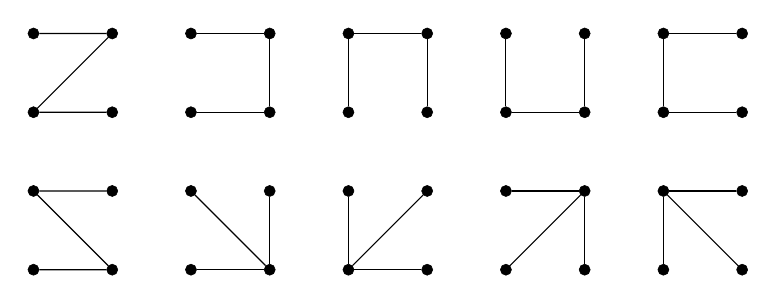
\begin{tikzpicture}[
	vertex/.style={ circle, draw, very thin, fill, inner sep=0pt, minimum size=4pt },
	vertexg/.style={ black!40!white, circle, draw, very thin, fill, inner sep=0pt, minimum size=4pt },
	vertexo/.style={ circle, draw, very thin, inner sep=0pt, minimum size=4pt }
]

\node[vertex] at (0,0) (v1) {};
\node[vertex] at (1,0) (v2) {};
\node[vertex] at (1,1) (v3) {};
\node[vertex] at (0,1) (v4) {};
\draw (v2) to (v1) to (v3) to (v4);

\node[vertex] at (0,-2) (v1) {};
\node[vertex] at (1,-2) (v2) {};
\node[vertex] at (1,-1) (v3) {};
\node[vertex] at (0,-1) (v4) {};
\draw (v1) to (v2) to (v4) to (v3);

\node[vertex] at (2,0) (v1) {};
\node[vertex] at (3,0) (v2) {};
\node[vertex] at (3,1) (v3) {};
\node[vertex] at (2,1) (v4) {};
\draw (v1) to (v2) to (v3) to (v4);

\node[vertex] at (4,0) (v1) {};
\node[vertex] at (5,0) (v2) {};
\node[vertex] at (5,1) (v3) {};
\node[vertex] at (4,1) (v4) {};
\draw (v1) to (v4) to (v3) to (v2);

\node[vertex] at (6,0) (v1) {};
\node[vertex] at (7,0) (v2) {};
\node[vertex] at (7,1) (v3) {};
\node[vertex] at (6,1) (v4) {};
\draw (v4) to (v1) to (v2) to (v3);

\node[vertex] at (8,0) (v1) {};
\node[vertex] at (9,0) (v2) {};
\node[vertex] at (9,1) (v3) {};
\node[vertex] at (8,1) (v4) {};
\draw (v2) to (v1) to (v4) to (v3);

\node[vertex] at (2,-2) (v1) {};
\node[vertex] at (3,-2) (v2) {};
\node[vertex] at (3,-1) (v3) {};
\node[vertex] at (2,-1) (v4) {};
\draw (v1) to (v2) to (v3);
\draw (v2) to (v4);

\node[vertex] at (4,-2) (v1) {};
\node[vertex] at (5,-2) (v2) {};
\node[vertex] at (5,-1) (v3) {};
\node[vertex] at (4,-1) (v4) {};
\draw (v2) to (v1) to (v4);
\draw (v1) to (v3);

\node[vertex] at (6,-2) (v1) {};
\node[vertex] at (7,-2) (v2) {};
\node[vertex] at (7,-1) (v3) {};
\node[vertex] at (6,-1) (v4) {};
\draw (v4) to (v3) to (v2);
\draw (v1) to (v3);

\node[vertex] at (8,-2) (v1) {};
\node[vertex] at (9,-2) (v2) {};
\node[vertex] at (9,-1) (v3) {};
\node[vertex] at (8,-1) (v4) {};
\draw (v3) to (v4) to (v1);
\draw (v2) to (v4);

\end{tikzpicture}
